%
% $Id: slides.tex 4228 2006-06-21 21:55:12Z jjamor $
%
%
% Compilar a .pdf con LaTeX (pdflatex)
% Es necesario instalar Beamer (paquete latex-beamer en Debian)
%

%
% Gr�ficos:
% Los gr�ficos pueden suministrarse en PNG, JPG, TIF, PDF, MPS
% Los EPS deben convertirse a PDF (usar epstopdf)
%

\documentclass{beamer}
\usetheme{Warsaw}
\usebackgroundtemplate{
\includegraphics[width=\paperwidth]{format/opensistemas-bg.png}}
\usepackage[spanish]{babel}
\usepackage[latin1]{inputenc}
\usepackage{graphics}
\usepackage{amssymb} % Simbolos matematicos

%\definecolor{libresoftgreen}{RGB}{162,190,43}
%\definecolor{libresoftblue}{RGB}{0,98,143}

%\setbeamercolor{titlelike}{bg=libresoftgreen}

%% Metadatos del PDF.
\hypersetup{
  pdftitle={CACert: A Community-driven Certification Authority},
  pdfauthor={Juanjo Amor},
  pdfcreator={OpenSistemas},
  pdfproducer=PDFLaTeX,
  pdfsubject={Open Source},
}
%%

\AtBeginSection[]
{
  \begin{frame}<presentation>
    \frametitle{Index}
    \tableofcontents[current]
  \end{frame}
}


\begin{document}

%% \renewcommand{\pause}{}

\title{CACert}
\subtitle{A Community-driven Certification Authority}
\institute{jjamor@opensistemas.com\\
OpenSistemas}
\author{Juanjo Amor}
\date{29 Abril 2011}

\frame{
\maketitle
\begin{center}

\includegraphics[width=6cm]{format/gsyc-open-urjc}
\end{center}
}


% Si el titulo o el autor se quieren acortar para los pies de p�gina
% se pueden redefinir aqu�:
%\title{Titulo corto}
%\author{Autores abreviado}


%% LICENCIA DE REDISTRIBUCION DE LAS TRANSPAS
\frame{
~
\vspace{4cm}

\begin{flushright}
{\tiny
(cc) 2011 Juanjo Amor and Wikipedia\\
  Some rights reserved. This work licensed under Creative Commons\\
  Attribution-ShareAlike License. To view a copy of full license, see\\
  http://creativecommons.org/licenses/by-sa/3.0/ or write to\\
  Creative Commons, 559 Nathan Abbott Way, Stanford,\\
  California 94305, USA.\\

%  Este documento (o uno muy similar) está disponible en \\
%  \url{http://gsyc.escet.urjc.es/~jjamor/}
}
\end{flushright}
}
%%

\section{About Opensistemas}

%%%%%%%%%%%%%%%%%%%%%%%%%%%%%%%%%%%%%%%%%%%%%%%%%%%%%%%%%%%%%%

\begin{frame}
\frametitle{About Opensistemas}
\begin{center}
Opensistemas is an {\LARGE international} company \pause highly {\LARGE specialized} \pause in
offering global {\Huge IT solutions} \pause based on {\Huge Open Source} and {\Huge Linux} platforms.
\end{center}
\end{frame}

\begin{frame}
\frametitle{About Opensistemas}
\begin{itemize}
\item Our Vision:
\pause
To become the international leader in Open Source Technologies.
\pause
\item Our Mission:
\pause
Apply our knowledge of the opportunities offered by Open Source to deliver
effective solutions and innovation to our customers while promoting the
professional development of our employees and building value for 
shareholders.
\pause
\item Our Values:
\pause
\begin{itemize}
\item Deliver effective solutiosn to our customers.
\item Corporate social responsibility.
\item Commitment to Open Source.
\item Ethics and Respect for individuals.
\item Research and Innovation.
\item Teamwork.
\item Commitment to the development of a society connected by information
and knowledge.
\end{itemize}
\end{itemize}
\end{frame}

\begin{frame}
\frametitle{About Opensistemas}
\begin{center}
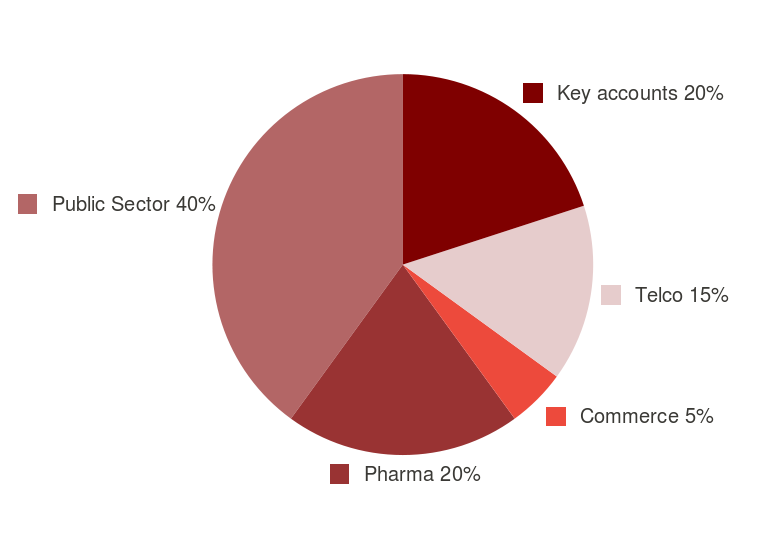
\includegraphics[width=9cm]{figs/opensistemas-markets}
\end{center}
\begin{center}
Our Markets
\end{center}
\end{frame}

\begin{frame}
\frametitle{About Opensistemas}
\begin{center}
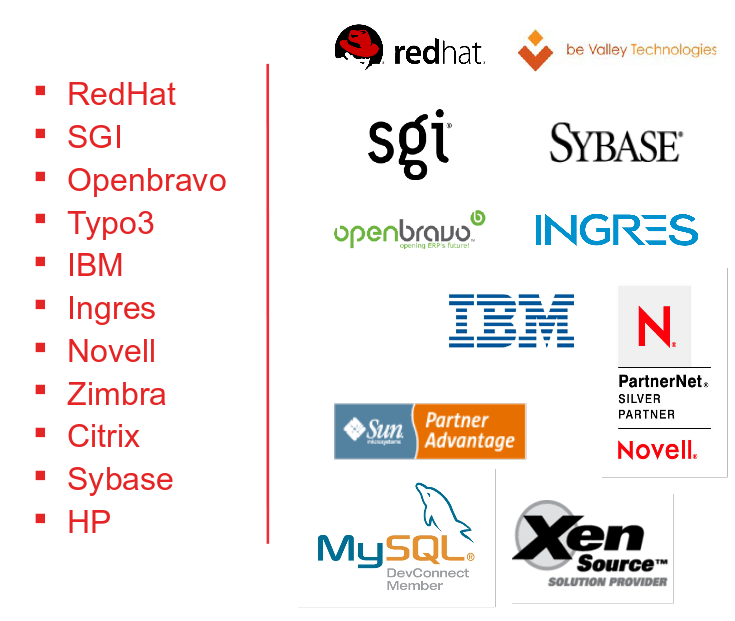
\includegraphics[width=7cm]{figs/opensistemas-partners}
\end{center}
\begin{center}
Our Partners
\end{center}
\end{frame}

\begin{frame}

\frametitle{About Opensistemas}
\begin{center}
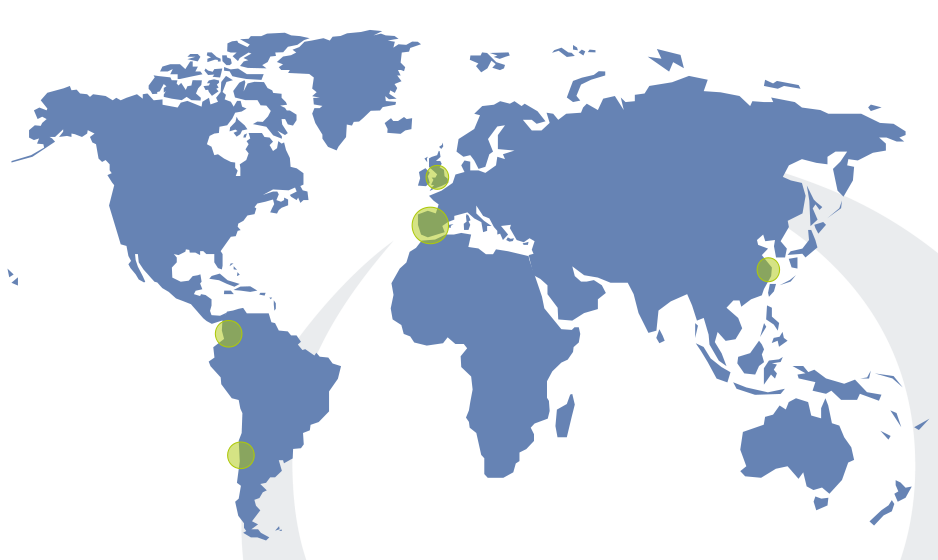
\includegraphics[width=9cm]{figs/opensistemas-worldmap}
\end{center}
\begin{center}
{\small Opensistemas is present in nine locations over five countries: Spain (Madrid, Valencia, Barcelona, Sevilla, Zaragoza), Chile (Santiago), Colombia (Bogot�), United Kingdom (London) and China (Shanghai).}
\end{center}
\end{frame}

\begin{frame}

\frametitle{About Opensistemas}
{\Huge Contact Information}
\begin{itemize}
\item www.opensistemas.com
\item info@opensistemas.com
\item +34 902 107 396
\end{itemize}
\end{frame}

\section{The PKI}

\begin{frame}
\frametitle{PKI concepts}

PKI meaning...
\pause
\begin{itemize}
\item PKI = Public Key Infrastructure
\pause
\item {\em a set of hardware, software, people, policies, and procedures needed to create, manage, distribute, use, store, and revoke digital certificates}
\end{itemize}

\pause

PKI components...
\pause
\begin{itemize}
\item CA = Certification Authority
\pause
\item RA = Registration Authority
\pause
\item VA = Validation Authority
\pause
\item Public keys (person, server and authority certificates)
\pause
\item Policies and procedures
\end{itemize}

\end{frame}


\begin{frame}
\frametitle{PKI}
\begin{center}
\includegraphics[width=9cm]{figs/Public-Key-Infrastructure}
\end{center}
\begin{center}
{\small diagram of a public key infrastructure}
\end{center}
\end{frame}

\begin{frame}
\frametitle{PKI example 1: Standard CA}

Standard CAs such as Thawte, Verisign...
\pause
\begin{itemize}
\item CA: Joins the CA, RA, VA.
\pause
\item Our navigator trusts in signed certificates by that CA
\pause
\item The certificate chain informs browser about VA
\end{itemize}
\pause
\begin{center}
Example: Try to get certificate information by using Thawte SSL Ca
\end{center}
\end{frame}

\begin{frame}
\frametitle{PKI example 2: The FNMT CA}

Spanish FNMT CA
\pause
\begin{itemize}
\item CA: Joins CA and VA.
\pause
\item RA: Delegated to other institutions such as AEAT, city councils...
\pause
\item CA certificate is not directly recognized by standard browsers \pause so we should import CA certificates into it.
\pause
\item This is one of first certificates acknowledged for legally identifying people or enterprises in Spain.
\end{itemize}
\pause
\begin{center}
Example: Import FNMT certificate and then get its information.
\end{center}

\end{frame}

\begin{frame}
\frametitle{PKI example 3: The DGP CA}

Spanish DGP (Police) CA
\pause
\begin{itemize}
\item CA: At DGP headquarters
\pause
\item RA: At DGP DNIe offices
\pause
\item VA: Delegated to third parties (FNMT, for example)
\pause
\item This is the CA for spanish electronic ID (DNIe). Also acknowledged for legally identifying people.
\end{itemize}
\pause
\begin{center}
Example: Import DGP certificate and then get its information.
\end{center}

\end{frame}

\begin{frame}
\frametitle{Web of Trust}

Web of trust
\pause
\begin{itemize}
\item Concept created by PGP creator.
\pause
\item Instead of having a ``central'' CA, we can build a trust network of signed public keys.
\pause
\item If A signs B, and C trust A, then C could trust B.
\pause
\item CACert uses a variant of trust network...
\end{itemize}

\end{frame}

\section{CACert}

\begin{frame}
\frametitle{CACert PKI}

What is CACERT?
\pause
\begin{itemize}
\item A community-driven certificate authority.
\pause
\item CACERT issues public key certificates to public (server, people) freely.
\pause
\item Robot CA: \pause Certificates are automatically signed. \pause These certificates are considered weak because CAcert does not emit any information in the certificates other than the domain name or email address (the CommonName field in X.509 certificates).
\pause
\item Web of trust: \pause Meetings, Assurance points, Prospective Assurers and Assures.
\pause
\item Assured users can get, for example, email certificates with a complete CommonName field.
\end{itemize}

\end{frame}

\begin{frame}
\frametitle{CACert inclusion status}

Can we use CACert server certificates with some browser?
\pause
\begin{itemize}
\item Yes, we can import CA certificate and go\ldots
\pause
\item Yes, my Linux distro (Debian, etc) includes CA certificate in ca-certificates package.
\pause
\item No, my browser does not recognize the certificates and I cannot trust to a strange CA.crt file! (Like a self-signed certificate)
\pause
\item Although Mozilla started a process to include the certificate, an audit suspended the process, because CACert needed to improve their management system.
\end{itemize}

\end{frame}

\begin{frame}
\frametitle{CACert web of trust}

When you create a new CACert account:
\pause
\begin{itemize}
\item Only your email can be verified
\end{itemize}
\pause
By meeting other CACert assurers you can get some points:
\pause
\begin{itemize}
\item for including your real name to your account,\pause
\item to generate {\em better} certificates, and finally,\pause
\item to be also a CACert assurer.
\end{itemize}

\end{frame}

\begin{frame}
\frametitle{CACert web of trust}

Some rules:
\pause
\begin{itemize}
\item An assurer can issue you upto 35 points. \pause
\item You need at least 50 points to have your full name assured \ldots \pause so you need to be assured by, at least, two existing assurers \pause
\item With 100 points you can also be an assurer \pause
\item \ldots but you also need to pass an ``assurer challenge'' \pause
\end{itemize}

More rules: \pause
When you are promoted to assurer: \pause
\begin{itemize}
\item Initially, you can issue 10 points to other people, and get 2 {\em experience points} when you assure somebody \pause
\item After you got 10 experience points, then you can issue 15 points to others \pause \ldots \pause
\item When you got 50 experience points, then you can issue to others the maximum per session: 35 points \pause
\item But in any case, you can, if you want, to issue less points than your maximum \pause
\end{itemize}

\end{frame}

\begin{frame}
\frametitle{CACert client certificates}

A client certificate is used to:
\pause
\begin{itemize}
\item Identify yourself to a web site
\pause
\item Email signing
\pause
\item \ldots
\end{itemize}
\pause
When you create a CACert account, you can get client certificates:
\pause
\begin{itemize}
\item Only the email is certified (by using email-ping)
\pause
\item With 6 month expiration
\end{itemize}
\pause
When you are assured (50 points) you also get
\pause
\begin{itemize}
\item Name and email certified
\pause
\item 24 month expiration
\end{itemize}

\end{frame}
\begin{frame}
\frametitle{CACert server certificates}

A server certificate is used to:
\pause
\begin{itemize}
\item Secure website: identify a server to you
\end{itemize}
\pause
When you create a CACert account, you can get server certificates:
\pause
\begin{itemize}
\item With 6 month expiration
\end{itemize}
\pause
When you are assured (50 points) you also get
\pause
\begin{itemize}
\item 24 month expiration
\end{itemize}
\pause
In all cases, you need to be able to ping DNS name by receiven a postmaster email from DNS owner, and only website DNS name is assured, because CACert assurers are not able
verify legal owner.

\end{frame}

%% PENDIENTE
%% Pr�cticas: Crear cuenta en CACert, quien lo desea puede ser asegurado por el profesor y por otros aseguradores presentes (Miquel?)
%% Despu�s describiremos el procedimiento para hacer un certificado personal, con openssl y con el navegador. http://wiki.cacert.org/EmailCertificates
%% Por �ltimo, la pr�ctica de hacer un servidor seguro, creando un csr que yo devolver� como crt dentro del dominio libresoft.es 

\begin{frame}
\frametitle{Questions}

\begin{center}
\Huge{Questions?}
\end{center}

\end{frame}

\begin{frame}
\frametitle{Exercises}

Final exercises
\begin{enumerate}
\item Creating your CACert account.
\item Creating your email certificate, with browser and then with openssl
\item Creating a web certificate, with openssl and apache
\item Want to be assured?
\end{enumerate}

\end{frame}

\end{document}
